%% LyX 2.2.2 created this file.  For more info, see http://www.lyx.org/.
%% Do not edit unless you really know what you are doing.
\documentclass[english]{scrartcl}
\usepackage[T1]{fontenc}
\usepackage[latin9]{inputenc}
\usepackage{color}
\usepackage{babel}
\usepackage{pdfpages}
\usepackage{graphicx}
\usepackage[unicode=true,pdfusetitle,
 bookmarks=true,bookmarksnumbered=false,bookmarksopen=false,
 breaklinks=true,pdfborder={0 0 0},pdfborderstyle={},backref=false,colorlinks=true]
 {hyperref}
\hypersetup{
 linkcolor=blue,citecolor=blue,urlcolor=blue}
\usepackage{breakurl}

\makeatletter

%%%%%%%%%%%%%%%%%%%%%%%%%%%%%% LyX specific LaTeX commands.
%% A simple dot to overcome graphicx limitations
\newcommand{\lyxdot}{.}


%%%%%%%%%%%%%%%%%%%%%%%%%%%%%% User specified LaTeX commands.
\usepackage{mciteplus}

\makeatother

\begin{document}

\titlehead{FY2018 Farm Bill Suggestion}

\title{Biological Control of Coconut Rhinoceros Beetle Biotype G}

\author{Aubrey Moore, University of Guam}

\maketitle
\tableofcontents{}

\pagebreak{}
\begin{abstract}
A newly discovered biotype of coconut rhinoceros beetle (CRB-G) is
rapidly killing coconuts and other palms on Guam. Following a failed
eradication attempt, CRB-G proved hard to control because it is resistant
to Oryctes nudivirus (OrNV), which was previously used as the preferred
biological control agent for control of CRB outbreaks on Pacific Islands
and elsewhere.

The overall objective of this project is to stop the uncontrolled
outbreak on Guam. Pacific-based entomologists working on this problem
agree that the most feasible solution is to find a new isolate of
OrNV which is highly pathogenic to CRB-G. Foreign exploration has
already discovered an OrNV isolate from an infected CRB-G collected
in the Philippines. If laboratory bioassays indicate that this isolate
is pathogenic for CRB-G, it will be propogated and distributed throughout
Guam by autodissemination. All previous OrNV releases on Pacific Islands
resulted in immediate and sustained suppression of CRB damage to low
levels and prevented tree mortality. We hope to find an OrNV isolate
which will produce similar results.

Guam is currently experiencing an uncontrolled and unmonitored island-wide
CRB-G outbreak which was triggered by abundant CRB-G breeding sites
in the form of dead and dying vegetation left in the wake Typhoon
Dolphin which occured in May 2015. of a recent typhoon. Most of these
breeding sites are inaccessable to sanitation efforts, being either
in the jungle or on military land (which covers one third of Guam).
A positive feedback cycle has begun whereby large numbers of adult
beetles are killing large numbers of palms which become breeding sites
which generate even higher numbers of adults. Severe damage to Guam's
palms prompted the Governor of Guam to declared a state of emergency
in July 2017. 

Entomologists working on this problem agree that the most feasible
tactic to halt tree mortality and suppress damage to tolerable levels
is establishment of biological control using an isolate of OrNV which
is highly pathogenic to CRB-G. Concurrent with establishment of CRB-G
biocontrol, success of the project will be monitored in a quarterly,
island-wide tree health survey and incidence of OrNV infection will
be monitored in a subsample of all field collected CRB-G. 

If the Guam CRB-G infestation cannot be controlled, it is expected
that most palms on the island will be killed and CRB-G will spread
to other islands and beyond. If CRB-G invades smaller islands and
atolls where coconut is \emph{the tree of life}, a human tragedy will
ensue. On larger islands, coconut and oil palm industries will be
severely impacted. Attempts to organize a regional project in response
to CRB-G are underway.

\pagebreak{}
\end{abstract}

\section{Technical Approach}

Coconut rhinoceros beetle (CRB), \emph{Oryctes rhinoceros}, is a major
pest of palms. Adults bore into crowns to feed on sap. A palms maybe
killed if CRB feeding activity damages the meristem. But this rarely
happens at low CRB population densities. CRB grubs do no damage. They
feed on decaying vegetation with standing dead coconuts and fallen
coconut logs being favored sites. In addition, they can feed in many
type of organic matter including dead trees, green waste, saw dust,
manure, compost, and even in bags of commercially packaged soil \cite{moore2016movement}.

CRB was first detected on Guam in 2007. Following failure of an eradication
attempt using mass trapping and sanitation, the beetle spread to all
parts of the island within a few years. \emph{Oryctes} nudivirus (OrNV)
and green muscardine fungus (GMF), \emph{Metarhizium majus}, where
introduced as biological control agents. GMF was successfully established
and a 2015 survey indicated that between 10\% and 38\% of Guam's CRB
were infected by this fungus \cite{moore2015efficacy}. However, the
preferred biocontrol agent for CRB, namely OrNV failed to have any
effect. Prior to the OrNV biocontrol failure on Guam, releases on
other Pacific islands resulted in reduction in CRB damage by up to
90\% within a few moths with control lasting for 30 plus years \cite{bedford2013longterm}.

This lead us to discover that the population of coconut rhinoceros
beetles (CRB) recently established on Guam is genetically distinct
from other populations of this major palm pest and it is being referred
to as the CRB-G biotype \cite{marshall2015anew2,marshall2017anew}.
CRB-G is resistant to all available isolates of OrNV, previously the
most effective biocontrol agent for CRB, and it appears to have other
characteristics, which make it more invasive and harder to control
than other CRB biotypes. While there where no range expansions of
CRB for a quarter of a century (1980 to 2005), CRB is now on the move
with the invasion of Guam in 2007, the Port Moresby area of Papua
New Guinea in 2009, Oahu, Hawaii in 2013, and the Honiara area of
Guadalcanal, Solomon Islands in 2015. It is significant that all of
these new invasions involve CRB-G. Thus, CRB-G is a regional problem
which poses significant risks to Pacific island economies and ecosystems.
Concerned Pacific-based entomologists are attempting to raise support
for coordinated regional response to CRB-G \cite{jackson2015needfor,vaqalo2015anemerging,marshall2016whitepaper}.
APHIS supported this effort by hosting a meeting at the International
Congress of Entomology, Florida, 2016 \cite{moore2016meeting}. 

Guam is currently experiencing massive mortality of coconut palms
as the result of a CRB population explosion triggered by abundant
larval breeding sites left in the wake of a Typhoon Dolphin which
visited the island in May 2015. Many coconut palms were killed by
numerous adults emerging from decaying vegetation, most of which was
inaccessible to sanitation, being in the jungle and/or on military
land. Resulting dead, standing coconuts quickly turned into breeding
sites which are generating even higher numbers of CRB adults. This
type of positive feed back cycle has been observed elsewhere following
tropical storm damage, large-scale land clearing or war. An CRB outbreak
occurred in the Palau Islands immediately following WWII resulting
in about 50\% coconut palms being killed by CRB throughout the archipelago
and 100\% mortality on some of the smaller islands \cite{gressitt1953thecoconut}.
A similar outcome can be expected for Guam if the current outbreak
is not controlled. In addition spread of CRB-G to other islands and
beyond can be expected. CRB has already been intercepted on Saipan
Island, about 200 miles north of Guam. Severity of the Guam CRB-G
outbreak resulted in Guam's Governor Calvo declaring a state of emergency
in July 2017.

The overall objective of this project is to stop an uncontrolled and
unmonitored outbreak of CRB-G on Guam which is rapidly killing coconut
and and other palms. Entomologists working on this problem agree that
the most feasible solution is establishment of biological control
using an isolate of OrNV which is highly effective for CRB-G \cite{jackson2015needfor,vaqalo2015anemerging,marshall2016whitepaper}.

Financial assistance will facilitate:
\begin{enumerate}
\item hiring a post-doc entomologist to assist with this project and continued
support for a graduate research assistant at the University of Guam
\item continued support for operating an insect pathology laboratory at
the University of Guam to evaluate and propagate candidate biocontrol
agents discovered during foreign exploration
\item support for a quarterly island-wide coconut palm health survey for
Guam
\item continued support for organizing an international collaborative project
with the goal of discovering a strain of OrNV or other microbial biocontrol
agent which is highly pathogenic for CRB-G
\end{enumerate}
This project is aligned with FB Goal 6: \emph{Enhance Mitigation and
Rapid Response} and it builds on progress made with the support of
FB funds from FY2014 through FY2017.

\subsection{Objective 1: Find an OrNV Isolate which is Highly Pathogenic for
CRB-G}

\subsubsection{Foreign Exploration for an Effective Biocontrol Agent for CRB-G}

During January, 2017, Moore, Iriarte and Marshall did field work on
Negros Island, Philippines, were CRB-G coexists with other CRB biotypes.
The major objective was to find an effective biocontrol agent for
CRB-G and a secondary objective was to develop and test protocols
for further foreign exploration. DNA analysis of CRB and OrNV from
rhino beetle gut samples collected during the trip is being done by
Dr. Sean Marshall in his lab at AgResearch New Zealand. Bioassays
of any detected OrNV will be done at the University of Guam. Further
foreign exploration for an effective biocontrol agent for CRB-G is
contingent on results from this first expedition. A report of the
Negros expedition is included in the Prior Experience section.

\subsubsection{Regional Collaboration on CRB-G Management}

Moore will continue to work with collaborators at AgResearch New Zealand,
the Secretariat of the Pacific Community (SPC), and USDA-APHIS to
put together a regional collaboration with the objective of finding
an effective biocontrol agent for CRB-G.

\subsection{Objective 2: Establish Sustainable Biocontrol of CRB-G by Autodissemination}

If the OrNV isolate from the infected beetle collected on Negros Island,
Philippines does not prove to be pathogenic for Guam beetles in a
high dose lab bioassay, foreign exploration will continue until a
pathogenic isolate is found. Otherwise, introduction of the virus
into the Guam CRB population via auto-dissemination will commence.
Autodissemination is a proven method for rapid establishment of OrNV
as a self sustaining biocontrol agent in CRB populations. Healthy
CRB adults are dosed with OrNV and released from multiple points.
Before these beetles get sick, they spread the virus within the healthy
population during mating and visits to breeding sites.

OrNV will be propagated \emph{in vitro} (in insect cell culture) at
AgResearch New Zealand and also \emph{in vivo} (in live CRB-G) at
the University of Guam. Beetles for auto-dissemination will be field
collected from breeding sites and pheromone traps because this is
far more efficient than rearing beetles in the lab at the current
time. A subsample of field collected beetles will dissected for visual
detection of OrNV infection, and gut tissue will be preserved for
molecular testing at AgResearch.

Concurrent with auto-dissemination releases, laboratory bioassays
will be performed to quantify the toxic (LD50, LT50, etc.) and nontoxic
effects (fecundity, flight capability, etc.) of OrNV on CRB. There
will also be an attempt to increase virulence by cycling isolates
through several generations of beetles. Beetles used in bioassays
will be field collected and maintained in individual Mason jars for
at least a month prior to being used to make sure they are healthy.
Beetles used for auto-dissemination will flight tested an marked with
a unique number prior to release using the methods outlined in Moore
et al. 2017 \cite{moore2017judasbeetles}.

\subsection{Objective 3: Establish a Sustainable Coconut Palm Health Monitoring
System}

The CRB-G outbreak on Guam is currently unmonitored on an island-wide
basis. An island-wide pheromone trapping system, using about 1500
traps, was operated by the University of Guam from 2008 to 2014. This
monitoring system was transferred to the Guam Department of Agriculture
which abandoned the effort at the end of February, 2016. Currently,
many coconut palms are being killed by CRB-G. But, in the absence
of a monitoring system, we do not have an estimate of tree mortality
or whether or not the damage is increasing or decreasing.

Clearly, establishment of a monitoring system is necessary if we want
to evaluate success of the proposed biocontrol project, or any other
mitigation efforts. We intend to establish a quarterly coconut tree
health survey rather than re-establish pheromone trapping.

\subsubsection{Survey Method}

The Coconut Palm Health Survey will use the following methodology
to track changes in levels of damage caused by CRB-G.
\begin{itemize}
\item The survey will monitor at least 1,000 palms located throughout the
island. An aluminum tag with a unique identifier will be affixed to
each palm on the initial visit.
\item The free smart phone app, EpiCollect+ will be used to georeference
each palm, record a digital image, and record damage data. (We have
successfully used this free app for several localized palm health
surveys.)
\item The survey will be performed four times per year.
\item CRB damage will be recorded in 3 boolean data fields:
\begin{itemize}
\item Mortality: 1 if palm is dead; 0 otherwise
\item New damage: 1 if any of the 4 youngest fronds have V-shaped cuts;
0 otherwise
\item Old damage: 1 if any other fronds have V-shaped cuts; 0 otherwise
\end{itemize}
\end{itemize}

\subsubsection{Digital Image Analysis}

We propose to add a methods development component to the survey. CRB
damage symptoms in the form of V-shaped cuts in fronds are distinctive
and easy to see in digital images. Digital imagery has been used for
detection and monitoring of CRB. For example, Soloman Sar in Papua
New Guinea has developed a Rapid Damage Assessment System in which
geotagged images of palms are rated for damage severity. It may be
possible to automate detection and monitoring of CRB damage by training
a computer to detect V-shaped cuts in digital images of coconut palms.
We will test this idea using human classified image libraries as training
sets. If successful, we will program a Raspberry Pi 3 equipped with
a camera to detect and quantify CRB damage in real time. This small,
inexpensive CRB damage detector could be mounted on a drone or a conventional
vehicle for automated detection and monitoring of CRB and damage caused
by this pest.

\subsection{Timeline}

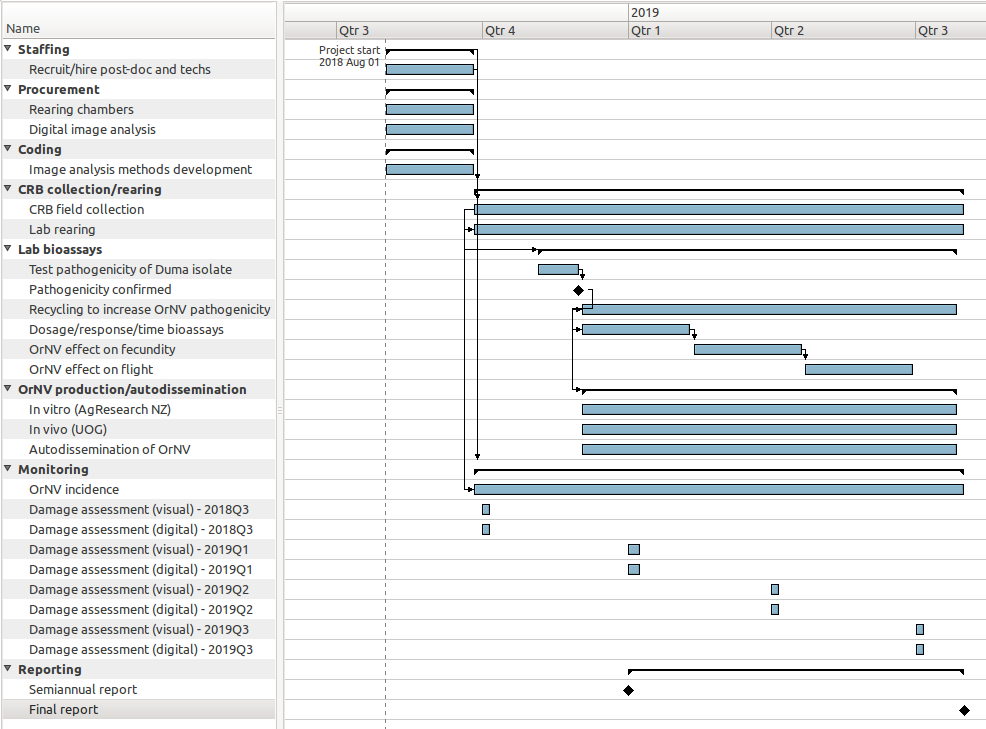
\includegraphics[width=1\textwidth,height=1\textheight,keepaspectratio]{timeline}

\pagebreak{}

\bibliographystyle{IEEEtran}
\phantomsection\addcontentsline{toc}{section}{\refname}\bibliography{lyz,temp}

\pagebreak{}

\section{Impacts and Benefits}
\begin{itemize}
\item Foreign exploration leading to discovery of a highly pathogenic strain
of OrNV or other microbial biocontrol agent for CRB-Guam could lead
to implementation of self sustaining population suppression and tolerable
damage levels on Guam and other islands invaded by CRB-G.
\item Loss of 50\% or more of Guam's palms may be prevented if an effective
biocontrol agent is found and released quickly.
\item Reduction in CRB population levels on Guam will reduce the risk of
accidental of the highly invasive CRB-Guam biotype to other Pacific
islands and elsewhere.
\item Development of image analysis methods may lead to a small, inexpensive,
automated CRB damage detector which could be mounted on a drone or
a conventional vehicle. This device could be used for early detection
or monitoring of CRB damage.
\end{itemize}
\pagebreak{}

\section{Prior Experience}

\subsection{Most Recent APHIS Farm Bill Progress Report, January 2017}

Please see following page.

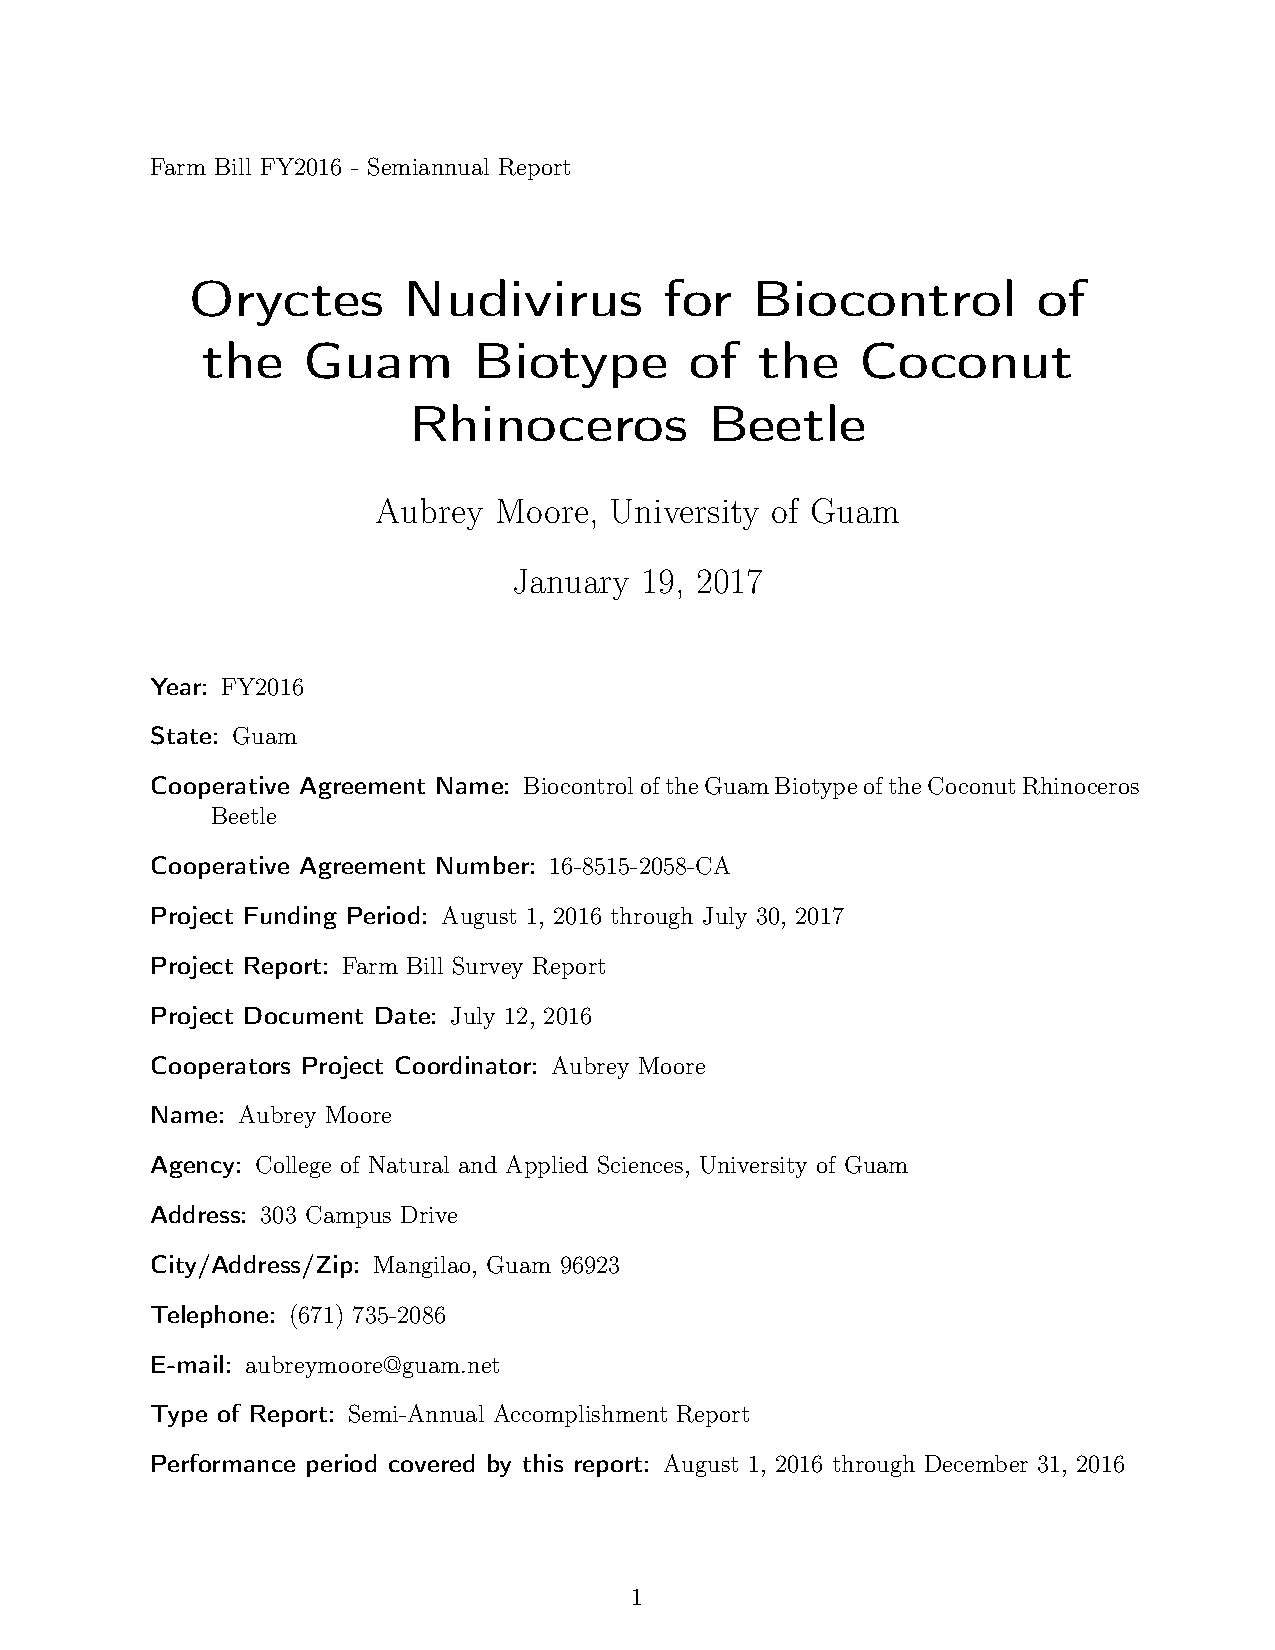
\includepdf[pages=-]{FB-REPORT1-FY2016}

\subsection{Report on Foreign Exploration for OrNV in Negros Island, Philippines,
January 2017}

Please see following page.

\includepdf[pages=-]{\string"AgR PH CRB PCR analysis Report_SM170615\string"}

\pagebreak{}

\section{Budget}

Please see following page.

\includepdf[pages=-]{\string"FY18-FB-budget \string"}
\end{document}
